% !Mode:: "TeX:UTF-8"

\chapter{}
\textbf{
We have a connected graph $G=(V,E)$, and a specific vertex $u\in V$. Suppose we compute a depth-first search tree rooted at $u$, and obtain a tree $T$ that includes all nodes of $G$. Suppose we then compute a breadth-first search tree rooted at $u$, and obtain the same tree $T$. Prove that $G=T$. (In other words, if $T$ is both a depth-first search tree and a breadth-first search tree rooted at $u$, then $G$ cannot contain any edges that do not belong to $T$.)
}


\hspace*{\fill} \\

Consider an example in figure~\ref{figure_0}. The tree $T$ in figure~\ref{figure_0} is the depth-first and breadth-first tree of ten vertex. 
\begin{figure}[!htbp]
  \centering
  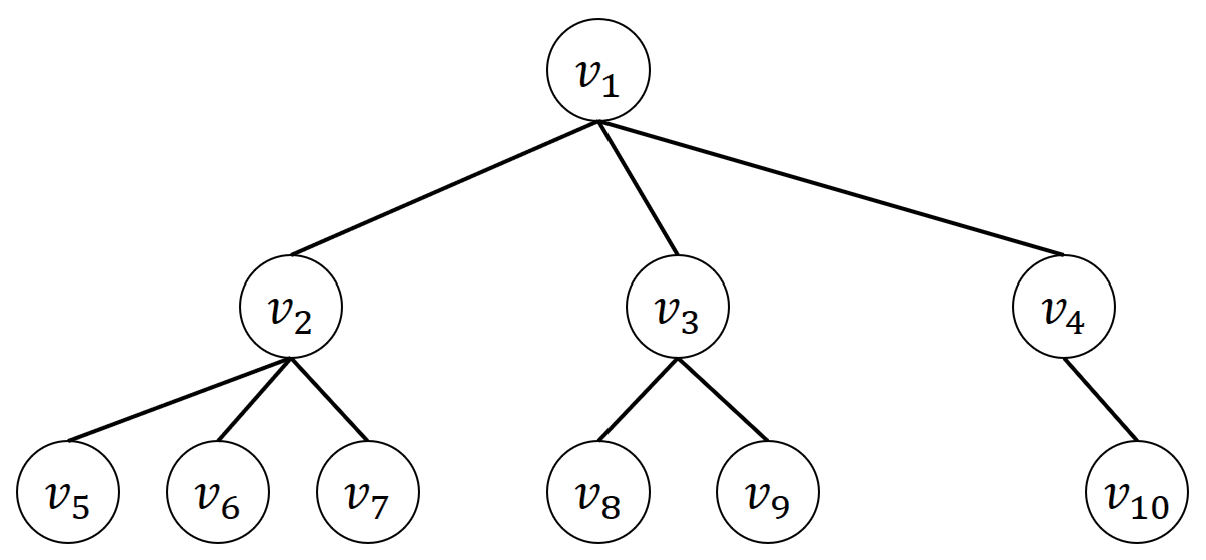
\includegraphics[width=0.5\textwidth]{figures/0.eps}\\
  \caption{depth-first and breadth-first tree}\label{figure_0}
\end{figure}
We firstly focus on breadth-first search tree.
We note two vertexes in the same layer(BFS search tree) and satisfy $v_i$ is before $v_j$ as $v_i \prec v_j$. We note prt($v$) as the parent node of $v$. Supposed that there is an edge $e$ which is not belong to $T$, then $e$ cannot across two or more layers in $T$. And $e$ cannot be $(\textrm{prt}(u),v)$ satisfying prt($u$) $\neq$ prt($v$) and $u\prec v$. Then $e$ must be the edge of the two following cases:

1) $e$ is between two vertexes $v_i$ and $v_j$ satisfying prt($v_i$)=prt($v_j$). As show in figure~\ref{figure_1_2}, in this case, the DFS tree is different from the BFS tree because $v_7$ will be access as the son of $v_6$ not the son of $v_2$ in the BFS tree.
\begin{figure}[!htbp]
\centering
\subfigure[BFS]{
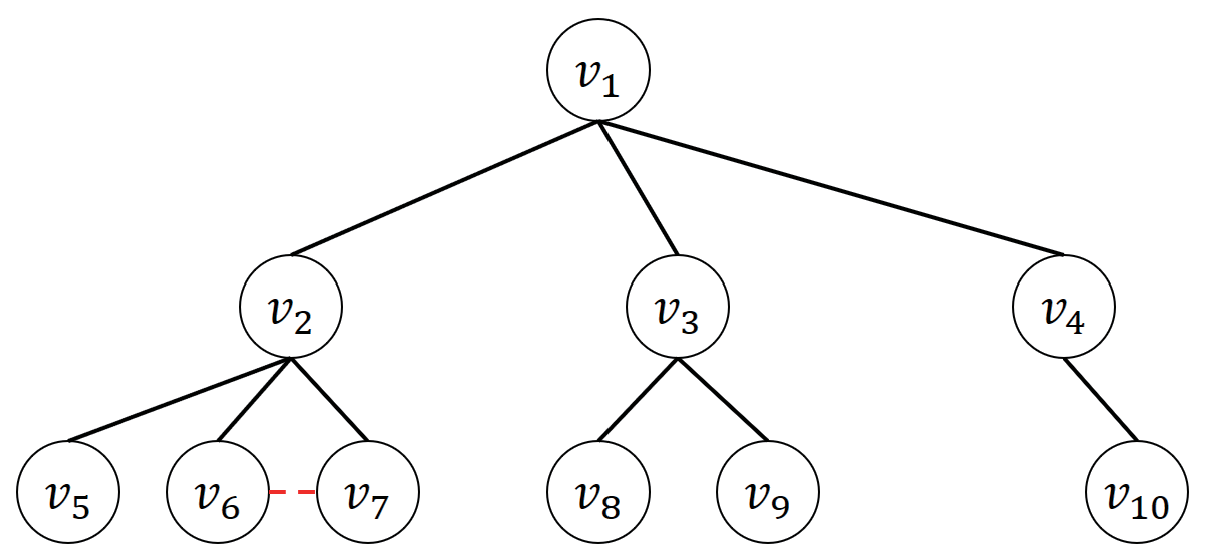
\includegraphics[width=0.3\textwidth]{figures/1.eps}}
\subfigure[DFS]{
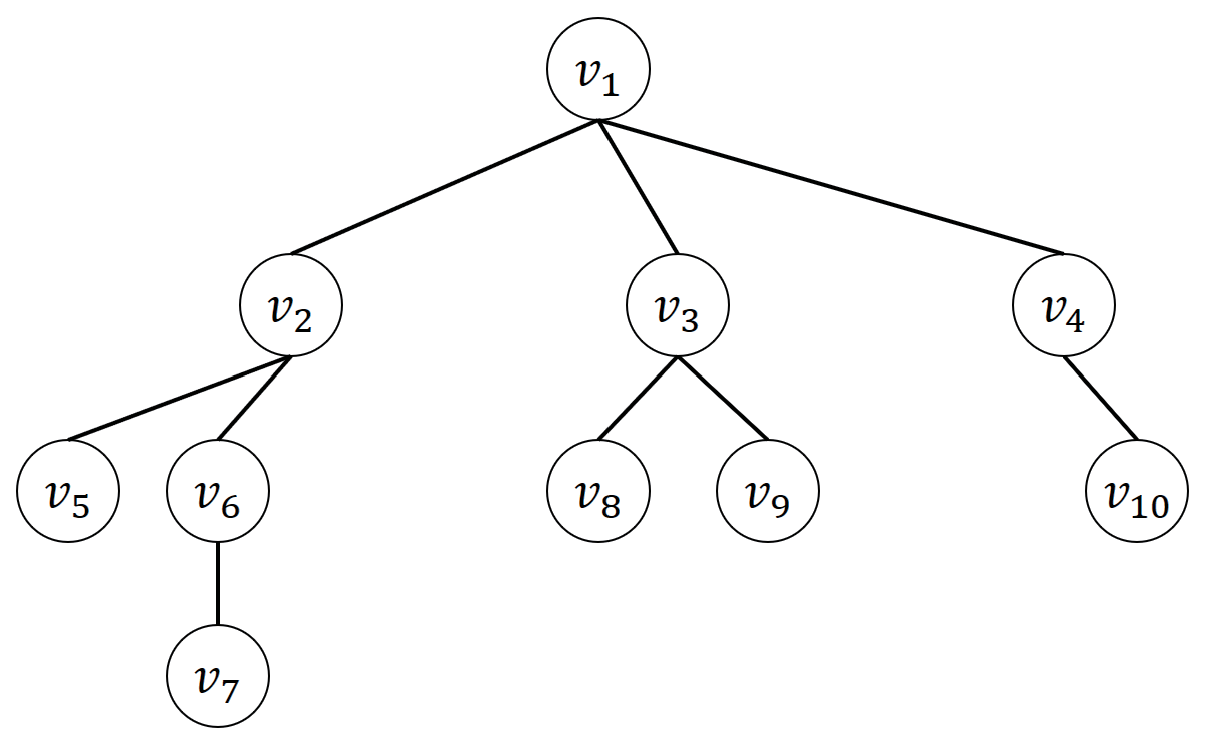
\includegraphics[width=0.3\textwidth]{figures/2.eps}}
\caption{$e$ is between two vertexes $v_i$ and $v_j$ satisfying prt($v_i$)=prt($v_j$)}\label{figure_1_2}
\end{figure}

2) $e$ is between two vertexes $v_i$ and $v_j$ satisfying prt($v_i$) $\neq$ prt($v_j$) and $v_j\prec v_i$. As show in figure~\ref{figure_3_4}, in this case, the DFS tree is different from the BFS tree because $v_3$ will be access as the son of $v_7$ not the son of $v_1$ in the BFS tree.
\begin{figure}[!htbp]
\centering
\subfigure[BFS]{
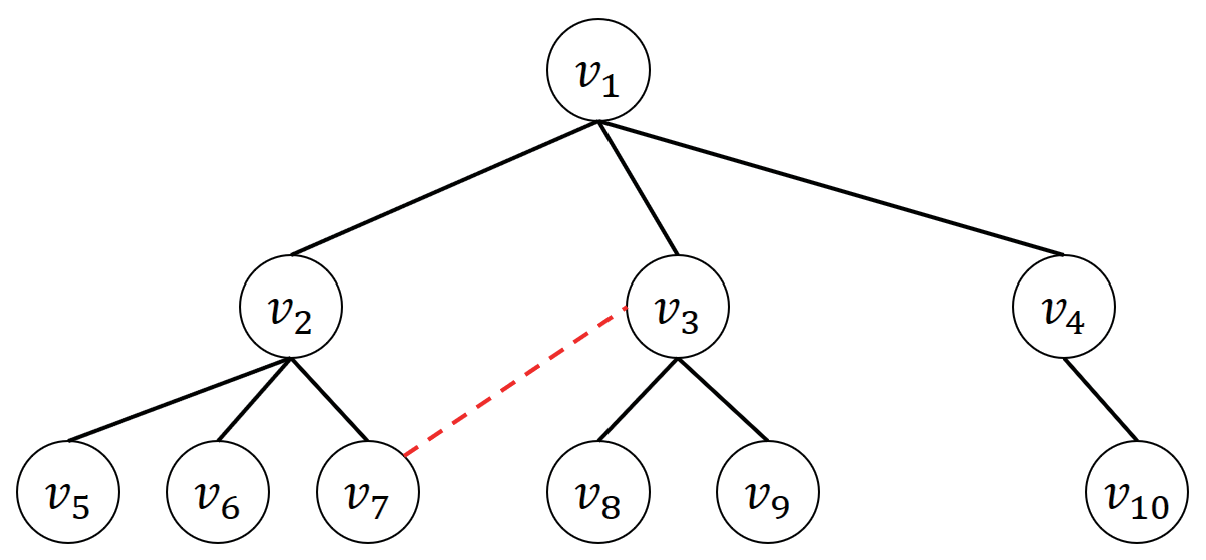
\includegraphics[width=0.3\textwidth]{figures/3.eps}}
\subfigure[DFS]{
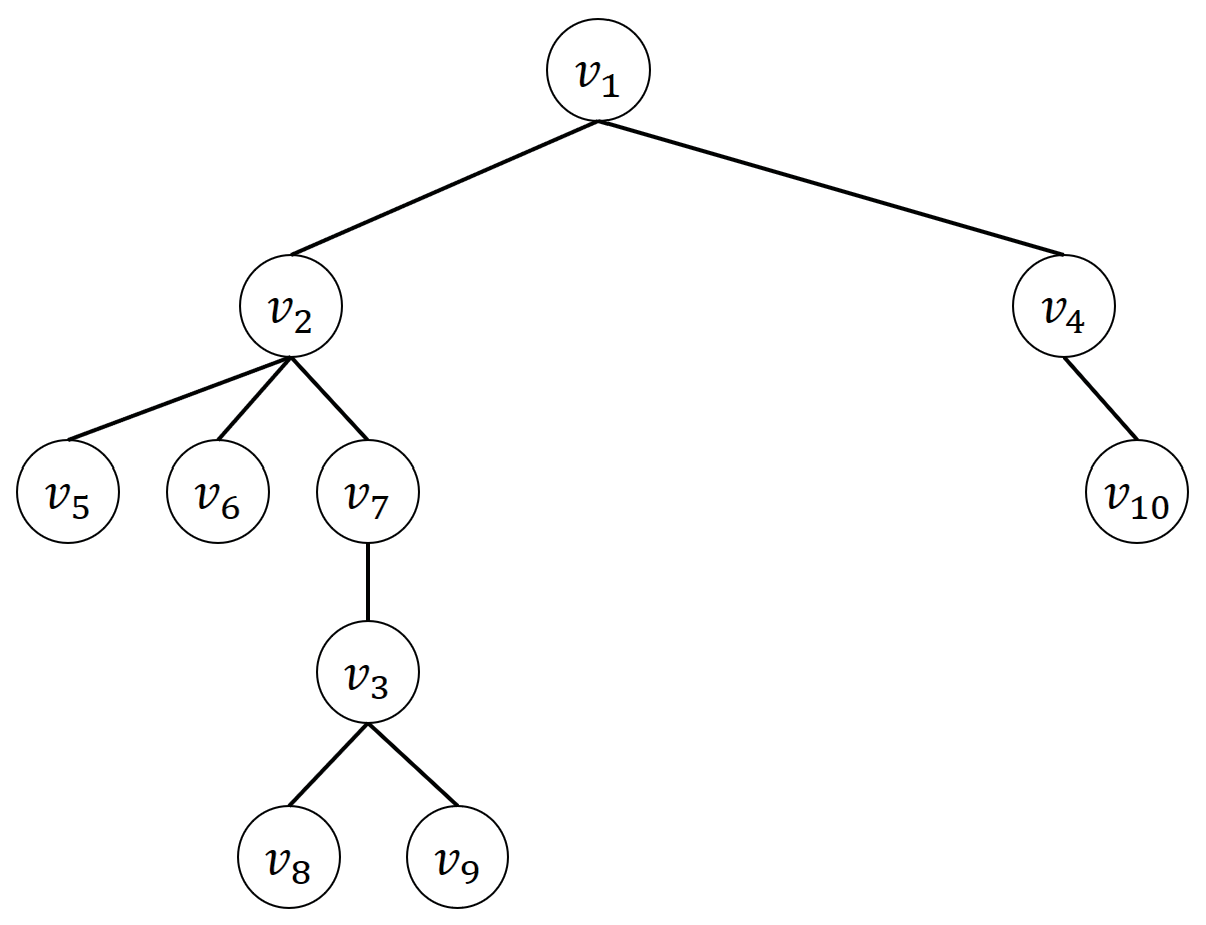
\includegraphics[width=0.3\textwidth]{figures/4.eps}}
\caption{$e$ is between two vertexes $v_i$ and $v_j$ satisfying prt($v_i$) $\neq$ prt($v_j$) and $v_j\prec v_i$}\label{figure_3_4}
\end{figure}

